\chapter{Implementation Plan}

\section{Framework Architecture}
We build our framework as a layer in top of the i5Cloud. The framework interact with the Openstack API to manage the instances that are running on the cloud. Figure \ref{fig:Framework Architecture} shows the architecture. The framework uses Apache Hama computing framework since it offers us both MapReduce and the BSP programming models. We use the MapReduce for the blocking and distribution phases, and we use the BSP based Pregel for the matching phase.
  
\begin{figure}[H]
\centering

\includegraphics {figures/chapter4/Framework_Layered_architecture.eps}  
\caption{Framework Architecture}
\label{fig:Framework Architecture}
\end{figure}

\section{i5Cloud Test bed}
i5Cloud is cloud computing platform hosted by the database and information systems chair in RWTH Aachen. The goal of i5Cloud is to provide infrastructure as a service (IaaS) and Platform as a service (Paas) for diverse applications and services \footnote{\url{http://dbis.rwth-aachen.de/cms/projects/i5cloud} accessed at 26.6.2013}.

The first version i5Cloud 0.1 used Sun Enterprise server with Sun SPARC T5240 architecture. The current version i5Cloud 0.2 uses Sun server with Sun Fire x4450 architecture. This server system can expand to up to 24 processing cores, 256 GB of memory, and more than 2 TB of internal storage. i5Cloud 0.2 hosts the  OpenStack\footnote{\url{http://www.openstack.org/}} open-source project for cloud infrastructure management. 

\subsection{OpenStack}
OpenStack is an open source software that provide infrastructure as service(Iaas). it consists of many components for managing the cloud resources (processing, storage, and networking resources). The components are Nova fabric controller, Swift salable redundant storage system, Cinder block storage, Quantum network management, Horizon dashboard, Keystone identification service and Glance image service. 

\section{Hama}
 Apache Hama is a pure BSP (Bulk Synchronous Parallel) computing framework on top of HDFS (Hadoop Distributed File System) for massive scientific computations such as matrix, graph and network algorithms. Hama focuses on general BSP computations, so it is not only for graphs.
The overall architecture of Hama is illustrated in Figure \ref{fig:Framework Architecture} . Hama has a layered architecture consisting of three components: Hama Core for providing many primitives to matrix and graph computations, Hama Shell for interactive user console, and Hama API. The Hama Core component also determines the appropriate computation engine\cite{SYK*10}. 

Hama supports three computation engines: MapReduce, BSP (Bulk Synchronous Parallel), and Dryad. The MapReduce is used for matrix computations, while BSP and Dryad are commonly used for graph computations. The main difference between BSP and Dryad is that BSP gives high performance with good data locality, while Dryad provides highly flexible computations with the fine control over the communication graph\cite{SYK*10}.

\begin{comment}
\begin{figure}[H]
\centering
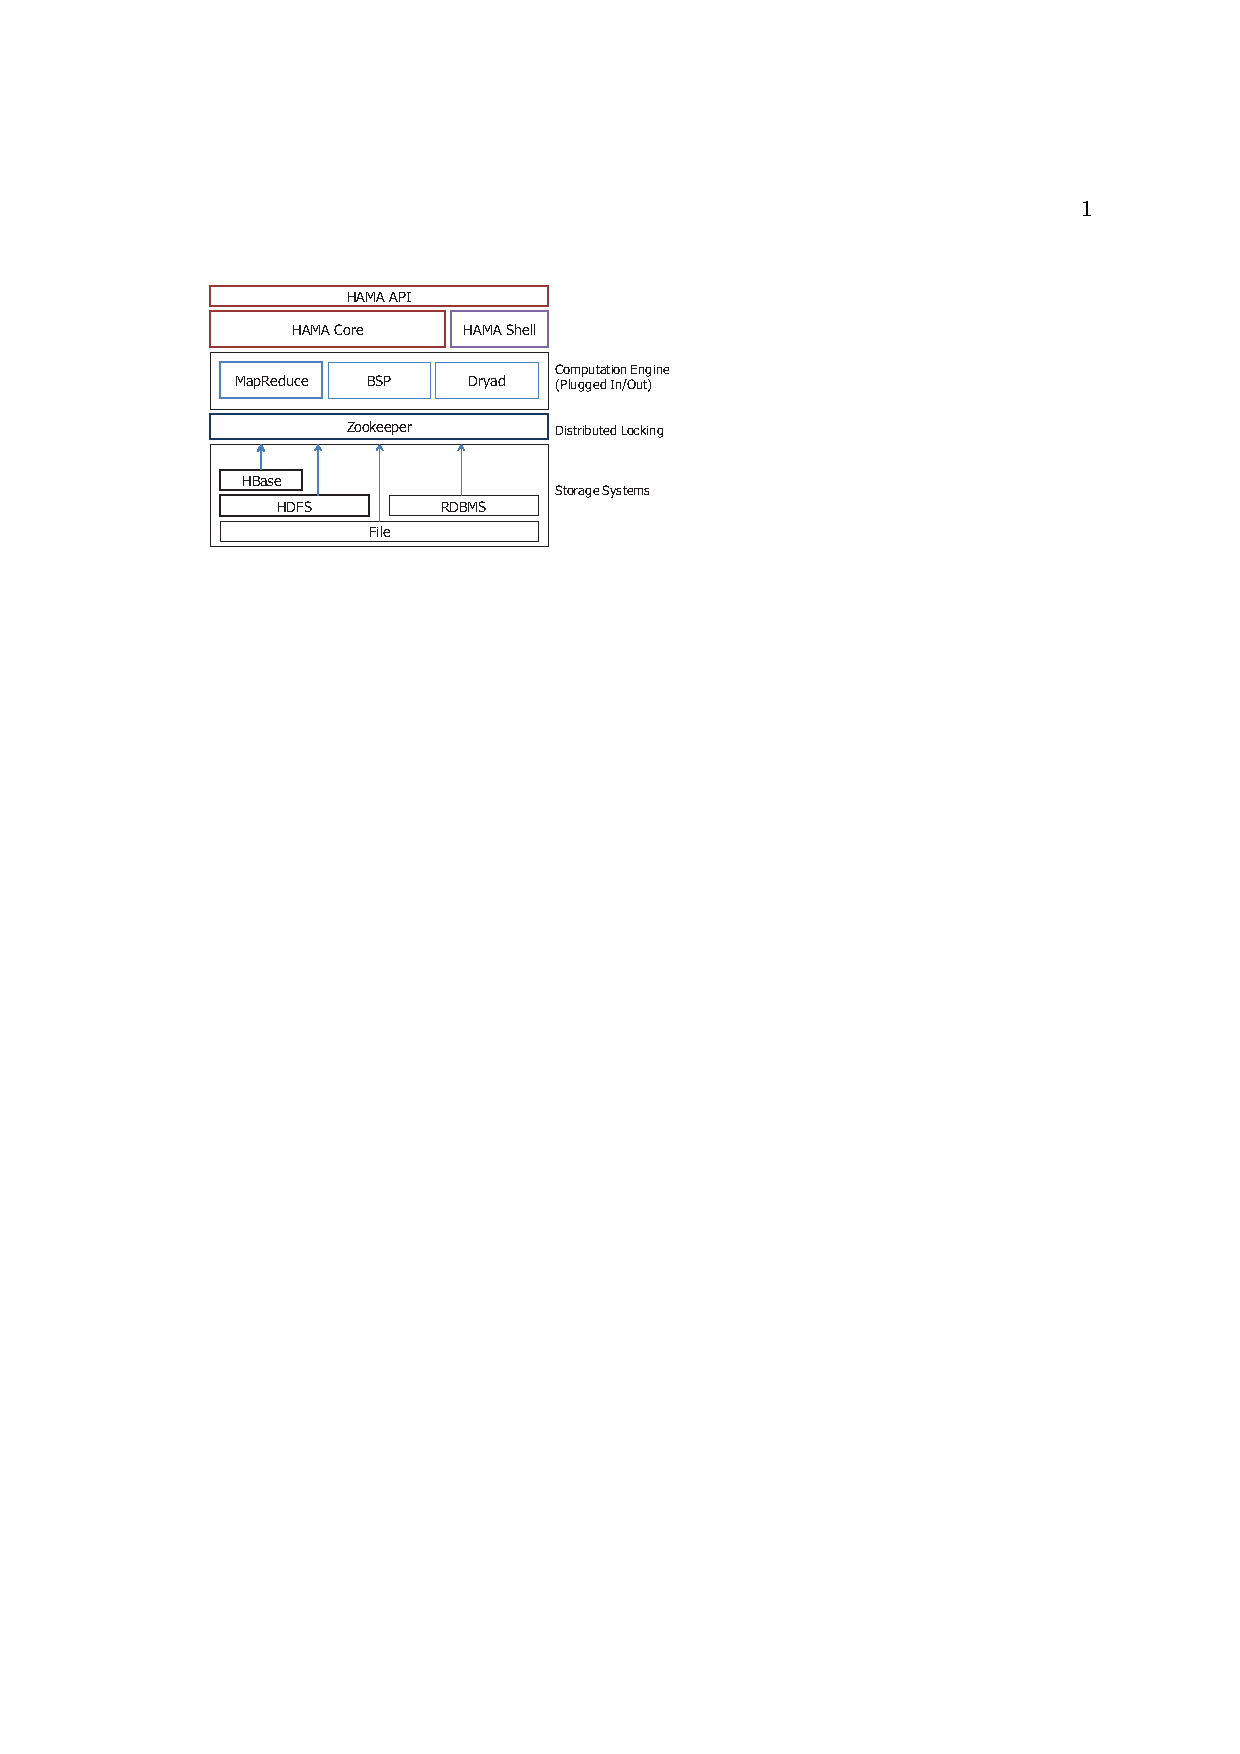
\includegraphics[page=1,trim = -10mm 203mm 0mm 45mm, clip]{figures/chapter4/fig_HAMA_clipping}  
\caption{Hama Architecture(\cite{\cite{SYK*10})}}
\label{fig:HAMAArchitecture}
\end{figure}
\end{comment}

\section{SimMetrics}
SimMetrics is a similarity measures library. it provide many of the attribute based similarity measures that we need to implement like cosine, Jaccard, Levenstein, etc. 